\documentclass [xcolor=svgnames, t] {beamer} 
\usepackage[utf8]{inputenc}
\usepackage{booktabs, comment} 
\usepackage[absolute, overlay]{textpos} 
\usepackage{pgfpages}
\usepackage[font=footnotesize]{caption}
\useoutertheme{infolines} 

\AtBeginSection[]{
  \begin{frame}
  \vfill
  \centering
  \begin{beamercolorbox}[sep=8pt,center,shadow=true,rounded=true]{title}
    \usebeamerfont{title}\insertsectionhead\par%
  \end{beamercolorbox}
  \vfill
  \end{frame}
}


%\definecolor{brownbrown}{RGB}{56, 28, 0}
%\definecolor{brownred}{RGB}{228, 0, 43}

%\setbeamercolor{title in head/foot}{bg=brownred, fg=brownbrown}
%\setbeamercolor{author in head/foot}{bg=myuniversity}
\setbeamertemplate{page number in head/foot}{}
\usepackage{csquotes}


\usepackage{amsmath}
\usepackage[makeroom]{cancel}


\usepackage{textpos}

\usepackage{tikz}

\usepackage{media9} 

\usetheme{Madrid}
%\definecolor{myuniversity}{RGB}{56, 28, 0}
%\usecolortheme[named=myuniversity]{structure}
\usepackage{tikz}



\title[Viscosidad]{Clase No.6: Propiedades de los fluidos}
\subtitle{Ley de viscosidad de Newton, tipos de fluidos y tipos de flujo}
\institute[]{Departamento de Ingenier\'ia Civil y Agr\'icola\\ Facultad de Ingenier\'ia  \\Universidad Nacional de Colombia - Sede Bogot\'a}
\titlegraphic{
\includegraphics[height=2.0cm]{escudoUnal.png}}
\author[LAM]{Luis Alejandro Morales \\ \href{https://lamhydro.github.io}{https://lamhydro.github.io}}


%\institute[]{Department of Earth, Environmental, and Planetary Sciences  \\Brown University}
\date{\today}


\addtobeamertemplate{navigation symbols}{}{%
    \usebeamerfont{footline}%
    \usebeamercolor[fg]{footline}%
    \hspace{1em}%
    \insertframenumber/\inserttotalframenumber
}

\begin{document}
\begin{frame}
\maketitle
\end{frame}


%%%%%%%%%%%%%%%%%%%%%%%%%%%%
\logo{\vspace{-0.2cm}
\includegraphics[height=0.8cm]{escudoUnal.png}~%
}
%%%%%%%%%%%%%%%%%%%%%%%%%%



\begin{frame}
\frametitle{Table of Contents}
\tableofcontents
\end{frame}


\section{Ley de viscosidad de Newton}
\begin{frame}{Ley de viscosidad de Newton}
\vspace{-0.5cm}
\begin{columns}
\column{0.5\textwidth}
\begin{block}{Viscosidad}
La \textbf{viscosidad} es una medida de la resistencia de un fluido a fluir (resistencia al corte). Esta determina la tasa de deformaci\'on de un fluido que es generada cuando este es sometido a un esfuerzo cortante $\tau$. Por ejemplo es mucho mas facil moverse en aire que en el agua, ya que esta ultima tiene una viscosidad 50 veces mas alta (ver Figura~\ref{visco0}). Mucho mas dificil es el movimiento en aceite que podria tener 300 veces mas viscosidad que el agua. 
\end{block}
\column{0.5\textwidth}
% Fig 2.23 Cengel 
\begin{figure}[h]
\centering
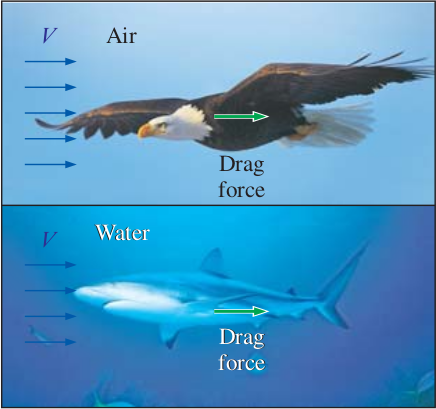
\includegraphics[width=0.9\textwidth]{visco0}
\caption{El fluido ejerce una fuerza de atrastre sobre el cuerpo en movimiento debido a la friccion causada por la viscosidad.}
\label{visco0}
\end{figure}
\end{columns}
\end{frame}


\begin{frame}{Ley de viscosidad de Newton}
Si consideramos un fluido que se mueve a una velocidad $u$ en un plano horizontal como resultado de una fuerza horizontal la cual produce un esfuerzo cortante, tenemos que el angulo de deformaci\'on $\delta \theta$ crece continuamente con el tiempo si $\tau$ se mantine (ver Figura~\ref{visco}).

% Fig 1.6 White
\begin{figure}[h]
\centering
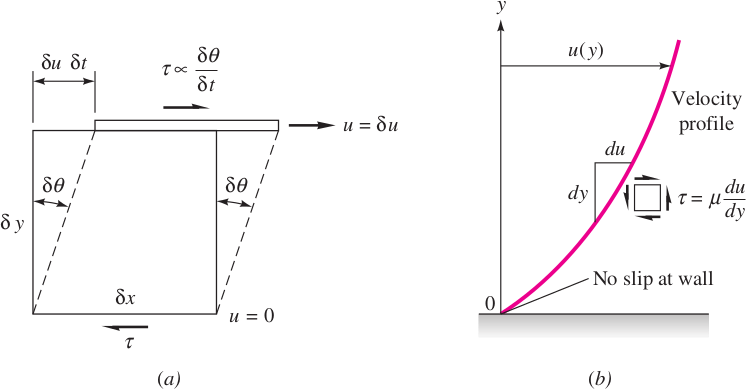
\includegraphics[width=7cm]{visco}
\caption{a)Deformacion de un fluido que flujo sobre una superficie horizontal a velocidad $u$ y  b) perfil de velocidades de fluido en la capa l\'imite.}
\label{visco}
\end{figure}

\end{frame}

\begin{frame}{Ley de viscosidad de Newton}
\vspace{-0.4cm}
% Fig 1.6 White
\begin{figure}[h]
\centering
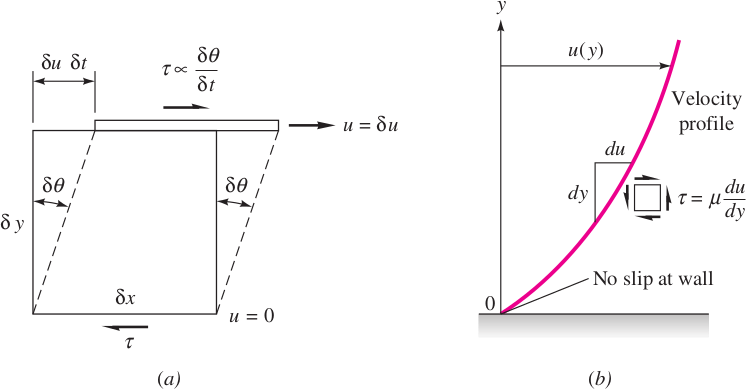
\includegraphics[width=7cm]{visco}
\caption{a)Deformacion de un fluido que flujo sobre una superficie horizontal a velocidad $u$ y  b) perfil de velocidades de fluido en la capa l\'imite.}
%\label{visco}
\end{figure}

Por lo tanto, en fluidos como el agua, el aceite o el aire, la tasa de deformacion se relaciona linealmente con el esfuerzo:
\begin{equation}
\tau \propto \frac{\delta \theta}{\delta t}
\label{vis1}
\end{equation}
\end{frame}

\begin{frame}{Ley de viscosidad de Newton}
\small
\vspace{-0.4cm}
% Fig 1.6 White
\begin{figure}[h]
\centering
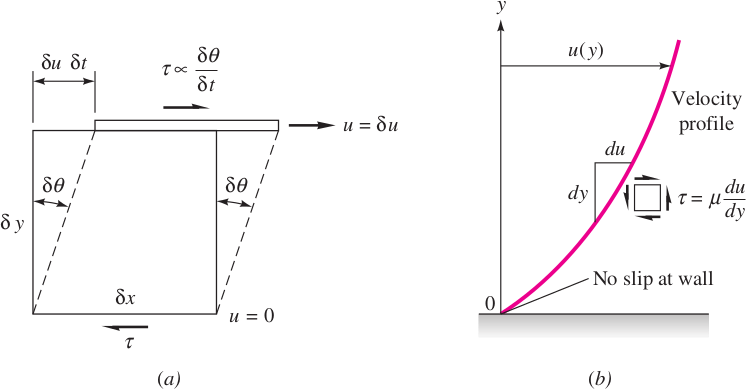
\includegraphics[width=6cm]{visco}
\caption{a)Deformacion de un fluido que flujo sobre una superficie horizontal a velocidad $u$ y  b) perfil de velocidades de fluido en la capa l\'imite.}
%\label{visco}
\end{figure}
\vspace{-0.4cm}
De la figura~\ref{visco}a:
$$
\tan \delta \theta = \frac{\delta u \delta t}{\delta y}
$$
En el limite infinitesimal cuando $\delta \theta$ se hace pequen\~no, $\tan \delta \theta \approx \delta \theta$ y la ecuacion anterior se comvierte en:
$$
\frac{d\theta}{dt}=\frac{du}{dy}
$$
la cual expresa la equivalencia entre la tasa de deformacion y el gradiente de velocidad.

\end{frame}

\begin{frame}{Ley de viscosidad de Newton}
\begin{block}{Ley de viscosidad de Newton}
Reemplazando en la ecuaci\'on~\ref{vis1} y teniendo en cuenta que la constante de proporcionalidad es el coeficiente de viscosidad $\mu$, conocido como viscosidad \emph{din\'amica} o \emph{absoluta}, tenemos:
\begin{equation}
\tau = \mu \frac{d \theta}{d t} = \mu \frac{d u}{d y}
\label{vis2}
\end{equation}
La ecuaci\'on~\ref{vis2} es conocidad como la Ley de viscosidad de Newton y es validad exclusivamente para flujos laminares.
\end{block}
Si analisamos el perfil de velocidades en la \textbf{capa limite} (ver Figura\ref{visco}b) la cual es la capa de fluido mas cercana a la placa solida inferior, la velocidad $u \approx 0$ y $\tau$ es m\'aximo en cercanias a la placa solida. Dicho fenomeno es conocido como la \textbf{condicion de no deslizamiento} en fluidos viscosos. 

\end{frame}

\begin{frame}{Ley de viscosidad de Newton}
\begin{block}{Dimensiones de la viscosidad}
$\mu$ tiene dimensiones ${FT/L^2}$ o ${M/LT}$, en SI son $kg/m.s$, en BG son $slugs/ft.s$ y en CGS son $g/cm.s = 1\ poise$. 
\end{block}
\end{frame}

\begin{frame}{Placas paralelas}
\vspace{-0.4cm}
Un problema  clasico es el flujo inducido entre una placa inferior fija y una placa superior que se mueve a una velocidad $\mathbf{V}$ (ver Figura~\ref{pla}). La distancia entre las placas es $h$ y dicho espacio esta ocupado por un fluido newtoniano. Si las placas son grandes, el movimiento permanente induce una distribucion de velocidad $u(y)$  (ver Figura~\ref{pla}) en donde $v=w=0$ y la aceleracion es zero. De acuerdo con lo anterior, a un balance de fuerza sobre un elemento de fluido resulta en un esfuerzo constante en cualquier punto del fluido. Por tanto la Equacion~\ref{vis2} se convierte en:

\begin{columns}
\column{0.6\textwidth}
% Fig 1.8 White
\begin{figure}[h]
\centering
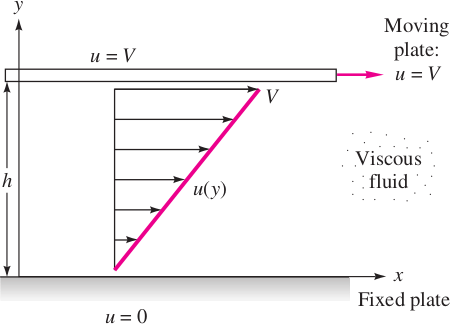
\includegraphics[width=5cm]{plate}
\caption{Flujo viscoso inducido por el movimiento relativo de dos placas paralelas.}
\label{pla}
\end{figure}

\column{0.4\textwidth}
$$
\frac{du}{dy}=\frac{\tau}{\mu}=\text{const}
$$
\end{columns}
\end{frame}

\begin{frame}{Placas paralelas}
Integrando esta ecuacion para $u$, tenemos
$$
u=a+by
$$
lo cual indica una distribucion lineal de la velocidad tal como se muestra en la Figura~\ref{pla} en donde $a$ y $b$ son constantes que se evaluan como:
$$
u= 
\begin{cases}
0 = a+b(0) & \quad \text{en}\ y=0 \\
V = a+b(h) & \quad \text{en}\ y=h 
\end{cases}
$$
de donde $a=0$ y $b=V/h$. Reemplazando en la ecuacion, el perfil de velocidades entre las placas esta dato por:
\begin{equation}
u=V\frac{y}{h}
\label{upl}
\end{equation}
\end{frame}

\begin{frame}{Variacion de la viscosidad con la temperatura}
La viscosidad es una propiedad termodinamica de los fluidos que depende de la presion $p$ y de la temperatura $T$. Sin embargo, la variacion de $\mu$ con respecto a la presion es menor, mientras qwue la variacion con respecto a la temperatura es significativa.
La viscosidad de un gas incrementa con la temperature. De acuerdo con esto existen dos leyes al respecto:
\begin{equation}
\frac{\mu}{\mu_0} \approx 
\begin{cases}
\left( \frac{T}{T_0} \right)^n & \quad \text{ley de potencia} \\
\frac{(T/T_0 )^{3/2}(T_0 + S)}{T+S} & \quad \text{ley de Sutherland} 
\end{cases}
\label{vist}
\end{equation}

donde $\mu_0$ es la viscosidad a una temperature absoluta $T_0$ (usualmente 273 K). Las constantes $n$ y $S$ son constantes ajustadas con base en datos. Por ejemplo para aire, $n\approx 0.7$ y $S\approx 110$ 
\end{frame}

\begin{frame}{Variacion de la viscosidad con la temperatura}
En liquidos, la viscosidad decrece con la temperatura de una forma casi exponencial $\mu \approx ae^{-bT}$. Con base en esta ecuacion esta expresion es derivada:
\begin{equation}
\ln \frac{\mu}{\mu_0} \approx  a + b \left(\frac{T_0}{T}\right)+ c\left(\frac{T_0}{T}\right)^2
\label{visf}
\end{equation}

en donde para agua con $T_0 = 273.16\ K$ y $\mu = 0.001792\ kg/(m.s)$, $a=-1.94$, $b=-4.80$ y $c=6.74$ con una  exactitud del $\pm 1$ \%.
\end{frame}


\section{Tipos de fluidos}
\begin{frame}{Tipos de fluidos}
\begin{block}{Fluidos newtonianos}
Son fluidos que se comportan de acuerdo con la ecuacion~\ref{vis2}.
\begin{equation}
\tau = \mu \frac{d \theta}{d t} = \mu \frac{d u}{d y}
\end{equation}

\end{block}
\end{frame}

\begin{frame}{Tipos de fluidos}
\begin{block}{Fluidos no newtonianos}
Fluidos que no siguen la equacion lineal ~\ref{vis2} son llamados \textbf{no newtonianos}. Mientras que en los flujos newtonianos la viscosidad es constante con el aumento del esfuerzo, en los fluidosno newtonianos la viscosidad cambia. Algunos tipos de fluidos no newtonianos son:
\end{block}
% Fig 2.26 Cengel
\begin{figure}[h]
\centering
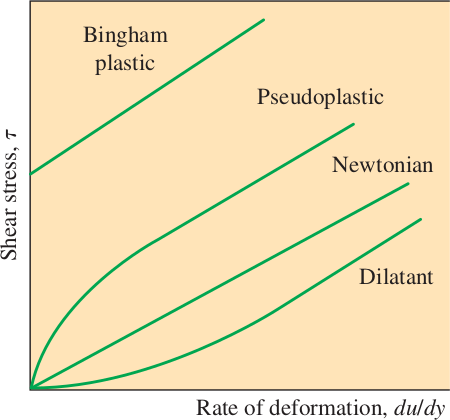
\includegraphics[width=8cm]{nonew}
\caption{Variacion del esfuerzo con la tasa de deformacion para fluidos newtonianos y no newtonianos.}
\label{nonew}
\end{figure}
\end{frame}

\begin{frame}{Tipos de fluidos}
\begin{block}{Tipos fluidos no newtonianos}
\begin{itemize}
\item \textbf{Dilatante}: Increase its resistencia cuando la tasa de deformacion incrementa.
\item \textbf{Seudoplastico}: La resistencia disminuye a altas tasas de deformacion. Por ejemplo: pintura y soluciones de polimeros. La pintura es gruesa antes de aplicarla pero se hace delgada cuando se aplica a una alta taza de deformacion.
\item \textbf{Bingham plastico}: Requieren un esfuerzo inicial antes de que inicie a fluir o deformarse. Por ejemplo: mayonesa, crema de dientes, lodos, salsa de tomate. La salsa de tomate no sale del recipiente a menos que se le aplique un esfuerzo inicial (se sacuda o se exprima el recipiente). 
\end{itemize}
\end{block}
\end{frame}

\section{Tipos de flujo}
\begin{frame}{Tipos de flujo}
\begin{block}{El Numero de Reynolds}
El numero de Reynolds $Re$ es un numero adimensional que caracteriza el movimiento de un fluido y se define como:
\begin{equation}
Re=\frac{\rho VL}{\mu}=\frac{VL}{\nu}
\label{re1}
\end{equation}
donde $V$ es la velocidad, $L$ es la longitud caracteristica del flujo y $\nu=\mu/\rho$  es la \textbf{viscosidad cinematica}. La ecuacion~\ref{re1} indica que $Re$ es la relacion de las fuerzas convectivas o inerciales y las fuerzas viscosas presentes en el fluido. De acuerdo con esto, $Re$ muy bajos significan flujos muy viscosos donde las fuerzas inerciales son despreciables. $Re$ moderados son flujos \textbf{laminares} que se mueven suavemente en capas paralelas. Un $Re$ alto es caracteristico de un flujo \textbf{turbulento}.  
\end{block}
\end{frame}

\end{document}

